% !TEX encoding = UTF-8 Unicode
%!TEX root = thesis.tex
% !TEX spellcheck = en-US
%%=========================================
\chapter{Results}
\label{chap:chapter4}
%Voltage running both Raspberry Pi and Tessel on: 5.015 V

In this chapter the results of all the experiments are presented.

Shown are the base power usage of both tested hardware platforms, i.e. the current drawn when no program is running.
This is done to see what amount of the current drawn when running the other experiments are due to the operation of the device.
The Raspberry Pi is shown to draw more than twice the current than the Tessel.

Next the approximate time for running the various programs on each software platform are tabulated.
These numbers are used to later find the average current drawn by a program run.

Then graphs of the current samples taken of each program on every platform are shown, to illustrate how a program run typically is.

In \fref{sec:avgcurrent}, the average current drawn per sample is shown, allowing for direct comparison with the results from \fref{sec:basepower}.
The results show that the Tessel draws far less current than the Raspberry Pi, but also that the Espruino VM draws less than io.js.
To explain this, the number of iterations per sample is shown in the section after, where it is shown that io.js manages to perform an order of magnitude more iterations per sample than the other platforms.

Lastly, the calculated average current drawn and power used by a single iteration in each program on every platform is shown.
Here it can be seen that despite drawing the most amount of current when running, io.js is the most efficient one per iteration.

\section{Base Power Usage}
\label{sec:basepower}
In figures \ref{fig:baserasp} and \ref{fig:basetessel}, power measurements of both hardware platforms running with no active program are graphed.
When the Raspberry Pi is running here, it is with a Linux distribution.
All the noise that can be seen is various background programs running, like networking and resource management.

With a sample set over 10 minutes, the average current drawn per sample is $0.378\si{\ampere}$ on the Raspberry Pi with no running program.

\begin{figure}[h!]
\centering
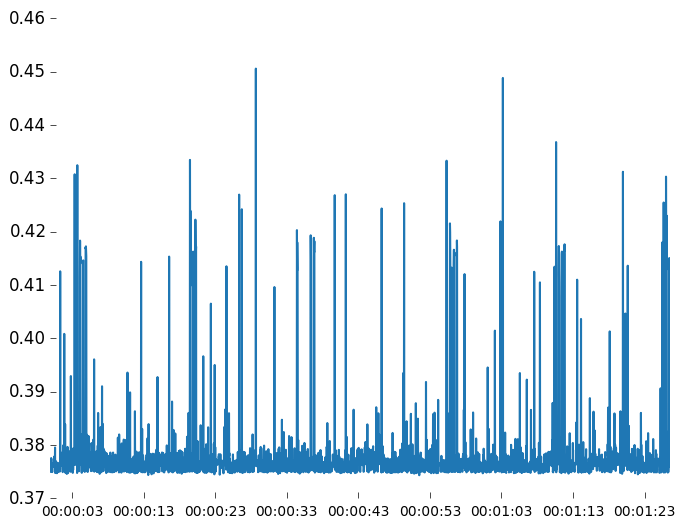
\includegraphics[scale=0.55]{fig/graphs/baseuse_rasp.png}
\caption{The Raspberry Pi running with no active program}
\label{fig:baserasp}
\end{figure}
\newpage

\begin{figure}[h!]
\centering
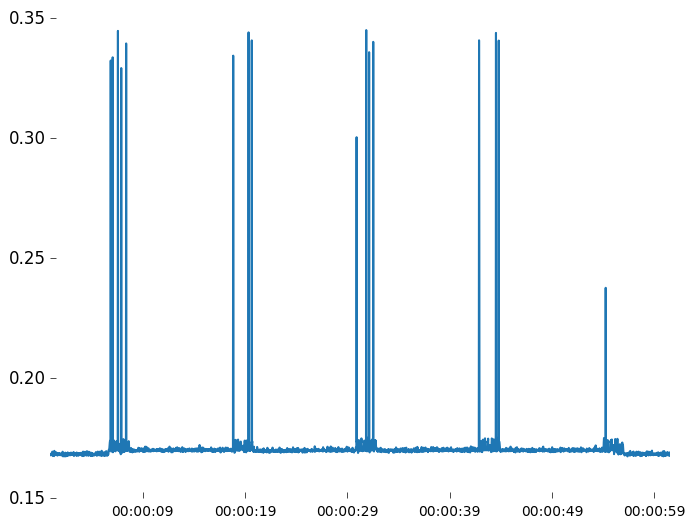
\includegraphics[scale=0.6]{fig/graphs/baseuse_tessel.png}
\caption{The Tessel running with no active program}
\label{fig:basetessel}
\end{figure}

In the Tessel graph, there is a lot less noise.
The high readings that can be seen, are from the WiFi-chip that is included.
About every 12 seconds, it checks the list it gathers of WiFi networks in range, to see if any of them are recognized.

With a sample set over 10 minutes, the average current drawn per sample is $0.162\si{\ampere}$ on the Tessel with no running program.

\section{Program time}
In \fref{tab:timedruns}, the approximate times of running the programs are gathered.
To note is the running time of the Left shift program on the Tessel, which is much higher than any other running time.
The closure program also systematically use longer time on every platform.
\begin{table}[h]
\centering
\begin{tabular}{ c  c  c  c  c }
 & Addition & Multiplication & Left shift & Closure \\ \midrule
 \rowcolor[gray]{.9}
 Espruino &  0m 48s & 0m 48s & 0m 49s & 1m 19s \\ 
 \rowcolor[gray]{.5}
 io.js  & 0m 3s & 0m 3s & 0m 3s & 0m 4s \\ 
 \rowcolor[gray]{.9}
 Tessel & 0m 19s & 0m 19s & 6m 12s & 2m 17s\\ 
 \bottomrule
\end{tabular}
\caption{Approximate time of each program}
\label{tab:timedruns}
\end{table}



\section{Current samples}
This section shows the results gathered by the multimeter, as described in \fref{sec:expsetup}.
The only manipulation done to this data is cutting it to not show the whole experiment, but rather just some interesting parts for illustration.

\begin{figure}[h!]
\centering
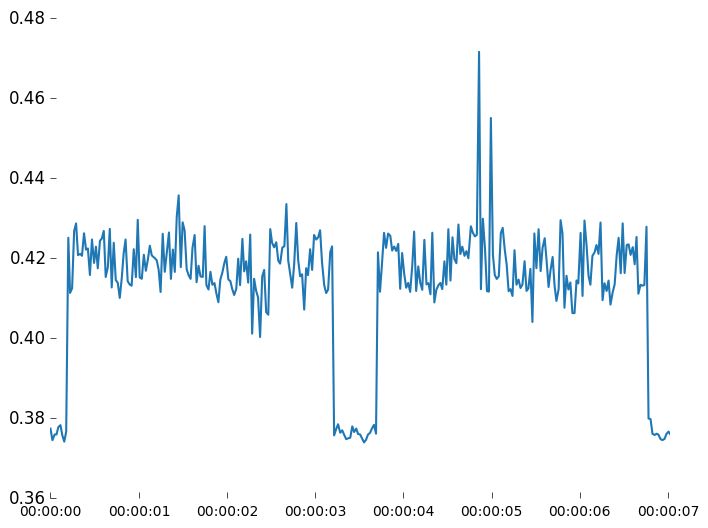
\includegraphics[scale=0.6]{fig/graphs/addition_iojs.png}
\caption{The addition program running in io.js on Raspberry Pi}
\label{fig:addraspio}
\end{figure}
\Fref{fig:addraspio} shows two complete runs of the addition program, which was shown in \fref{lst:add}, in io.js on the Raspberry Pi.
The dips in the readings are the sleep period between each run of the program.
As many parts of the OS is paused when the sleep command is issued, the spikes that could be seen in \fref{fig:baserasp} is not present between the program runs.


\begin{figure}[ht]
\centering
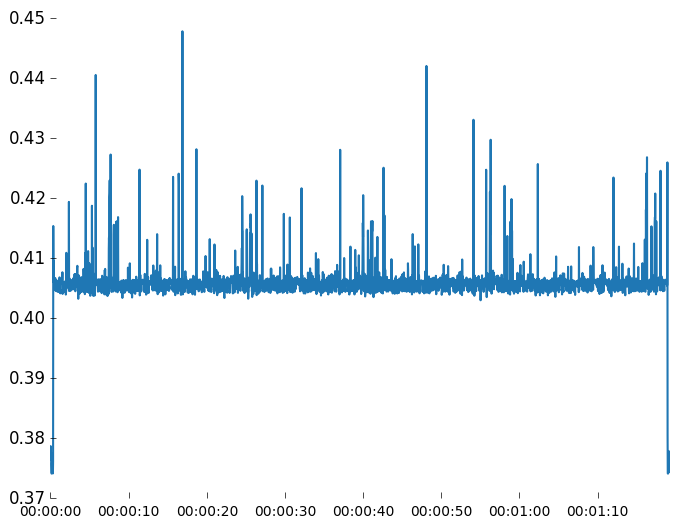
\includegraphics[scale=0.6]{fig/graphs/closure_espruino.png}
\caption{The closure program running in Espruino on Raspberry Pi}
\label{fig:closesp}
\end{figure}
Shown in \fref{fig:closesp}, is a single run of the closure program.
As the program running time is at about the same length as the run with no program shown in \fref{fig:baserasp}, the spikes here are similar to the graph when running with no program.
The dips, seen  are identical with \fref{fig:addraspio}

\clearpage

\begin{figure}[h!]
\centering
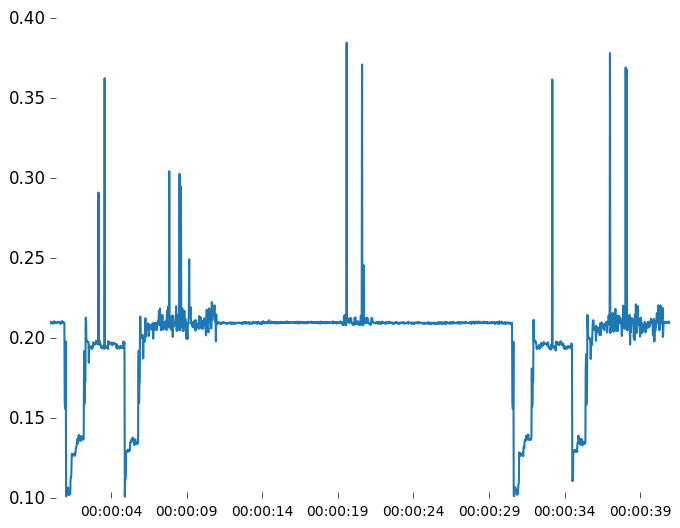
\includegraphics[scale=0.6]{fig/graphs/tessel_multi.png}
\caption{The multiplication program running on the Tessel 1}
\label{fig:multtes}
\end{figure}
In \fref{fig:multtes}, a single run of the multiplication program on the Tessel is shown, as well as the two power resets of the device on either side.
The WiFi chip turning on can also be seen in the middle of the graph.


\section{Average current drawn per sample}
\label{sec:avgcurrent}



\newcolumntype{A}{>{\columncolor[gray]{.9}}m{1.3cm}}
\newcolumntype{D}{>{\columncolor[gray]{.8}}m{1.3cm}}
\begin{table}[h!]
\centering
\begin{tabular}{c c}
    \begin{tabular}{c A}
    \multicolumn{2}{c}{Add}\\
    Espruino & 0.409 \si{\ampere} \\
    io.js & 0.419 \si{\ampere} \\
    Tessel & 0.203 \si{\ampere}
    \end{tabular} &
    
    \begin{tabular}{c A}
    \multicolumn{2}{c}{Multiplication} \\
    Espruino & 0.409 \si{\ampere}\\
    io.js & 0.419 \si{\ampere} \\
    Tessel & 0.203 \si{\ampere}
    \end{tabular} \\
& \\
    \begin{tabular}{c A}
    \multicolumn{2}{c}{Shift} \\
    Espruino & 0.409 \si{\ampere} \\
    io.js & 0.419 \si{\ampere} \\
    Tessel & 0.219 \si{\ampere}
    \end{tabular} &
    
    \begin{tabular}{c A}
    \multicolumn{2}{c}{Closure} \\
    Espruino & 0.406 \si{\ampere} \\
    io.js & 0.422 \si{\ampere} \\
    Tessel & 0.215 \si{\ampere}
    \end{tabular}
\end{tabular}
\caption{Average current drawn per sample}
\label{tab:avgcurrent}
\end{table}

\Fref{tab:avgcurrent} shows the average current drawn per sample of each program, with the same data as used in \fref{tab:results}.
As can be seen, io.js draws the most current per sample.

\section{Iterations per sample}
Using the number of samples taken in the experiments, the number of iterations is done per sample is shown in \fref{tab:iterpersample}.
These values are tied to how fast the programs run, as a program that runs for a longer time will be sampled more often, as the sample rate is constant.
\begin{table}[h!]
\centering
\begin{tabular}{c c}
\begin{tabular}{c A}
    \multicolumn{2}{c}{Add}\\
    Espruino & 4.8  \\
    io.js & 64.0 \\
    Tessel & 8.1
    \end{tabular} &
    
    \begin{tabular}{c A}
    \multicolumn{2}{c}{Multiplication} \\
    Espruino & 4.7\\
    io.js & 64.1\\
    Tessel & 7.8
    \end{tabular} \\
& \\
    \begin{tabular}{c A}
    \multicolumn{2}{c}{Shift} \\
    Espruino & 4.6 \\
    io.js & 63.9 \\
    Tessel & 0.7
    \end{tabular} &
    
    \begin{tabular}{c A}
    \multicolumn{2}{c}{Closure} \\
    Espruino & 3.0 \\
    io.js & 63.9 \\
    Tessel & 1.8
    \end{tabular}
\end{tabular}
\caption{Iterations per sample}
\label{tab:iterpersample}
\end{table}

\section{Energy use per iteration}

\newcolumntype{C}{>{\columncolor[gray]{.9}}m{1.3cm}}
\newcolumntype{D}{>{\columncolor[gray]{.8}}m{1.3cm}}
\begin{adjustwidth}{-1cm}{}
\begin{table}[ht]
\centering
\begin{tabular}{m{7cm} m{5cm} }
    \begin{tabular}{c C D C}
    & \multicolumn{3}{ c }{Add}  \\
    & Tessel & io.js & espruino  \\
    {\tiny Current (\si{\micro\ampere})} & 158.18 & 55.286 & 844.32  \\
    {\tiny Power (\si{\micro\watt})} & 793.27 & 277.26 & 4,234.3 \\
    \end{tabular} &

    \begin{tabular}{C D C}
    \multicolumn{3}{ c }{Multiplication} \\
    Tessel & io.js & espruino \\
    165.67 & 55.276 & 844.16 \\ 
    830.84 & 277.21 &  4,233.5 \\
    \end{tabular}\\

    & \\
    \begin{tabular}{c C D C}
    & \multicolumn{3}{ c }{Closure} \\
    & Tessel & io.js & espruino \\
    {\tiny Current (\si{\micro\ampere})} & 1,196.3 & 70.896 & 1347.9 \\
    {\tiny Power (\si{\micro\watt})} & 5,999.4 & 355.54 & 6,759.7
    \end{tabular} &
    
    \begin{tabular}{C D C}
    \multicolumn{3}{ c }{Shift} \\
    Tessel & io.js & espruino \\
    3,334.5 & 55.276 & 862.05 \\
    6,723 & 277.21 & 4,323.2
    \end{tabular}\\

\end{tabular}
\caption{Energy per iteration in loop}
\label{tab:results}
\end{table}
\end{adjustwidth}

In \fref{tab:results}, the calculated average current drawn and power used per iteration in each program is collected.
The values are shown in \si{\micro\ampere}, but as the number of iterations is 1,000,000, the values in the table is also representing the current drawn for the entire program run.
